%=============================================================================
% CHAPTER 2: THEORETICAL BACKGROUND
%=============================================================================

\clearpage

\chapter{Theoretical Background}

\section{Introduction}

Before I began designing my password strength evaluation tool, I first explored the theoretical and practical background of password security. Understanding how passwords are created, attacked, managed, and evaluated allowed me to identify the essential factors that determine their strength in real-world scenarios. This chapter summarises the key concepts, common attack methods, and established approaches to assessing password robustness, as well as the limitations of current practices.

In particular, I examine how users choose passwords, which psychological and usability factors influence those choices, and how attackers exploit predictable patterns. I also review existing metrics and tools for measuring password strength, including rule-based approaches, entropy-based models, and modern data-driven methods that leverage leaked password datasets. By outlining this foundation, the chapter motivates the design goals and requirements for my own evaluation tool.


\section{Role of Passwords in Our World}

Passwords serve as the primary mechanism for authentication in most systems people use, from email services to banking platforms, social networks, and cloud storage solutions. A password functions as a shared secret between the user and the system, serving as the first line of defence against unauthorised access. However, the effectiveness of this mechanism depends on password quality and how it is stored and verified by the system. Weak or reused passwords make it easier for attackers to compromise accounts, leading to identity theft, financial loss, data breaches, and large-scale compromise of online services.

In addition to attacks that directly guess or crack passwords, poor password practices---such as writing passwords on paper, sharing them between accounts, or using default credentials---further increase the risk. From an organizational perspective, compromised passwords can affect not only individual accounts but also critical infrastructure and sensitive business data.

Although advanced methods such as multi-factor authentication (MFA), hardware security keys, and biometrics are becoming more common, passwords still dominate due to their simplicity, low cost, and compatibility with existing systems. In many cases, they remain the fallback or recovery method even when stronger authentication is used. Figure~\ref{fig:auth_methods} illustrates the trade-off between adoption rate and security strength for the most common authentication methods.

\begin{figure}[H]
    \centering
    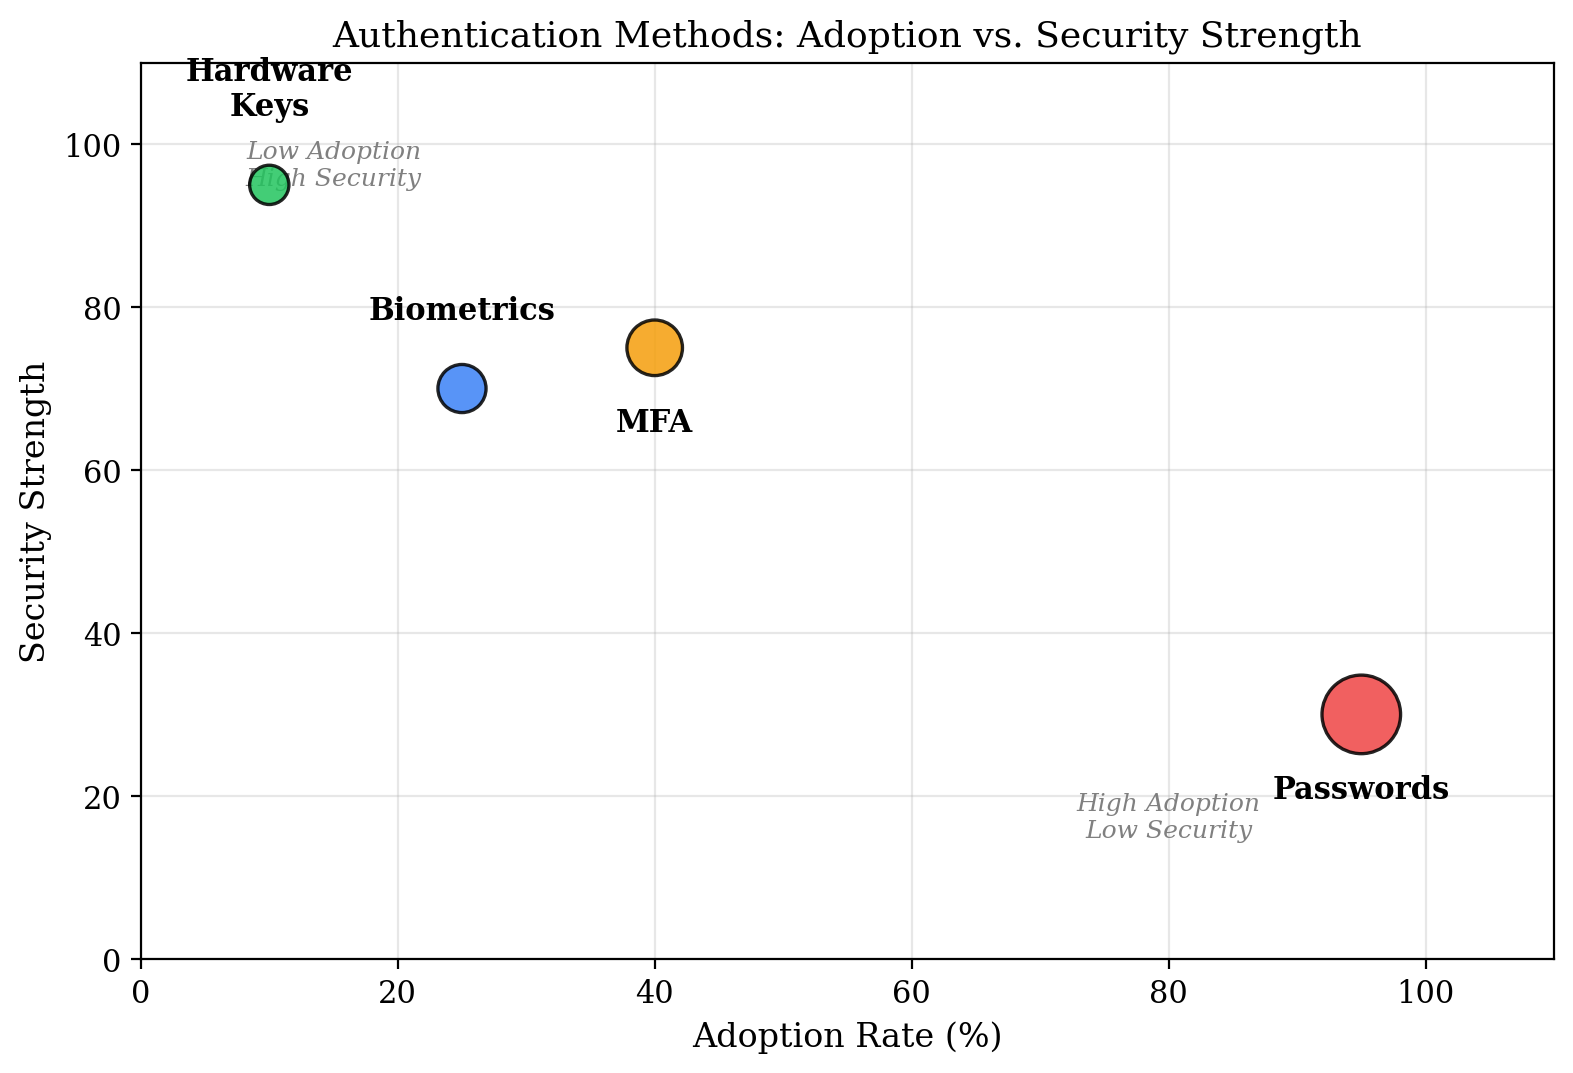
\includegraphics[width=0.85\textwidth]{figures/auth_methods_comparison.png}
    \caption{Comparison of authentication methods by adoption rate and security strength.}
    \label{fig:auth_methods}
\end{figure}

Therefore, improving password quality is still a crucial part of cybersecurity. This includes encouraging users to create strong, unique passwords and designing systems, such as the proposed password strength evaluation tool, that help users and administrators better understand and reduce the risks associated with weak passwords.

\section{Common Password Vulnerabilities}

During my research, I identified several factors that contribute to weak passwords. Table~\ref{tab:vulnerability_examples} summarises the most common vulnerability types, provides concrete examples, and links each to its impact on the password search space and the attack methods that exploit it.

\begin{table}[H]
\centering
\caption{Common password vulnerability types, examples, and their security impact.}
\label{tab:vulnerability_examples}
\begin{tabularx}{\textwidth}{>{\raggedright\arraybackslash}p{2.8cm} >{\raggedright\arraybackslash}p{2.5cm} >{\raggedright\arraybackslash}p{3cm} >{\raggedright\arraybackslash}p{3.5cm}}
\toprule
\textbf{Vulnerability Type} & \textbf{Example} & \textbf{Search Space Impact} & \textbf{Attack Method} \\
\midrule
Short length & \texttt{abc1} & $26^{4} \approx 457{,}000$ combinations & Brute-force (seconds) \\
\midrule
Lack of complexity & \texttt{password} & $26^{8} \approx 2 \times 10^{11}$ vs.\ $94^{8} \approx 6 \times 10^{15}$ & Dictionary attack \\
\midrule
Reused passwords & Same password on 5+ sites & One breach compromises all accounts & Credential stuffing \\
\midrule
Dictionary words & \texttt{sunshine2024} & Predictable structure: word + year & Dictionary with mutation rules \\
\midrule
Personal information & \texttt{John1995!} & Guessable via social engineering & Targeted dictionary attack \\
\bottomrule
\end{tabularx}
\end{table}

\begin{figure}[H]
    \centering
    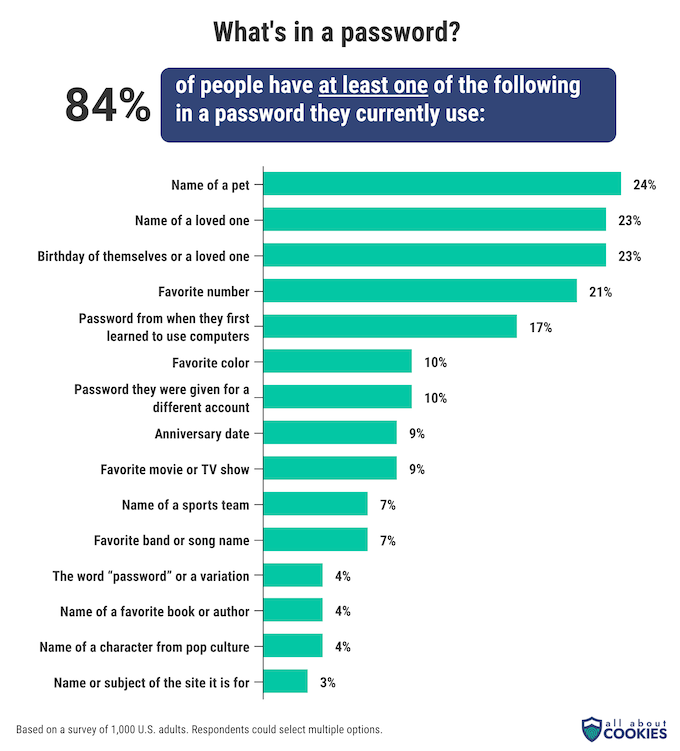
\includegraphics[width=0.85\textwidth]{figures/password_behaviour.png}
    \caption{User dangerous password behaviours.}
    \label{fig:password_behaviour}
\end{figure}

The fundamental problem with each of these vulnerabilities is that they reduce the effective search space an attacker must explore. A password that appears long and complex but follows a predictable pattern (such as a dictionary word with appended digits) can often be cracked faster than a shorter but truly random string, because attackers optimise their strategies by trying the most likely patterns first \cite{weir2009}.


\section{Mechanisms of Password Attacks}

Understanding how attackers attempt to compromise passwords is essential for designing effective evaluation criteria. This section describes the four principal categories of password attacks and explains how each motivates a specific dimension of the evaluation algorithm developed in this thesis.

\subsection{Brute-Force Attacks}

In a brute-force attack, the attacker systematically tries every possible combination of characters until the correct password is found. For a password of length $L$ drawn from a character set of size $N$, the total number of possible combinations is $N^{L}$. Modern hardware, particularly graphics processing units (GPUs), can attempt billions of guesses per second, making short passwords with small character sets trivially breakable.

\begin{figure}[H]
    \centering
    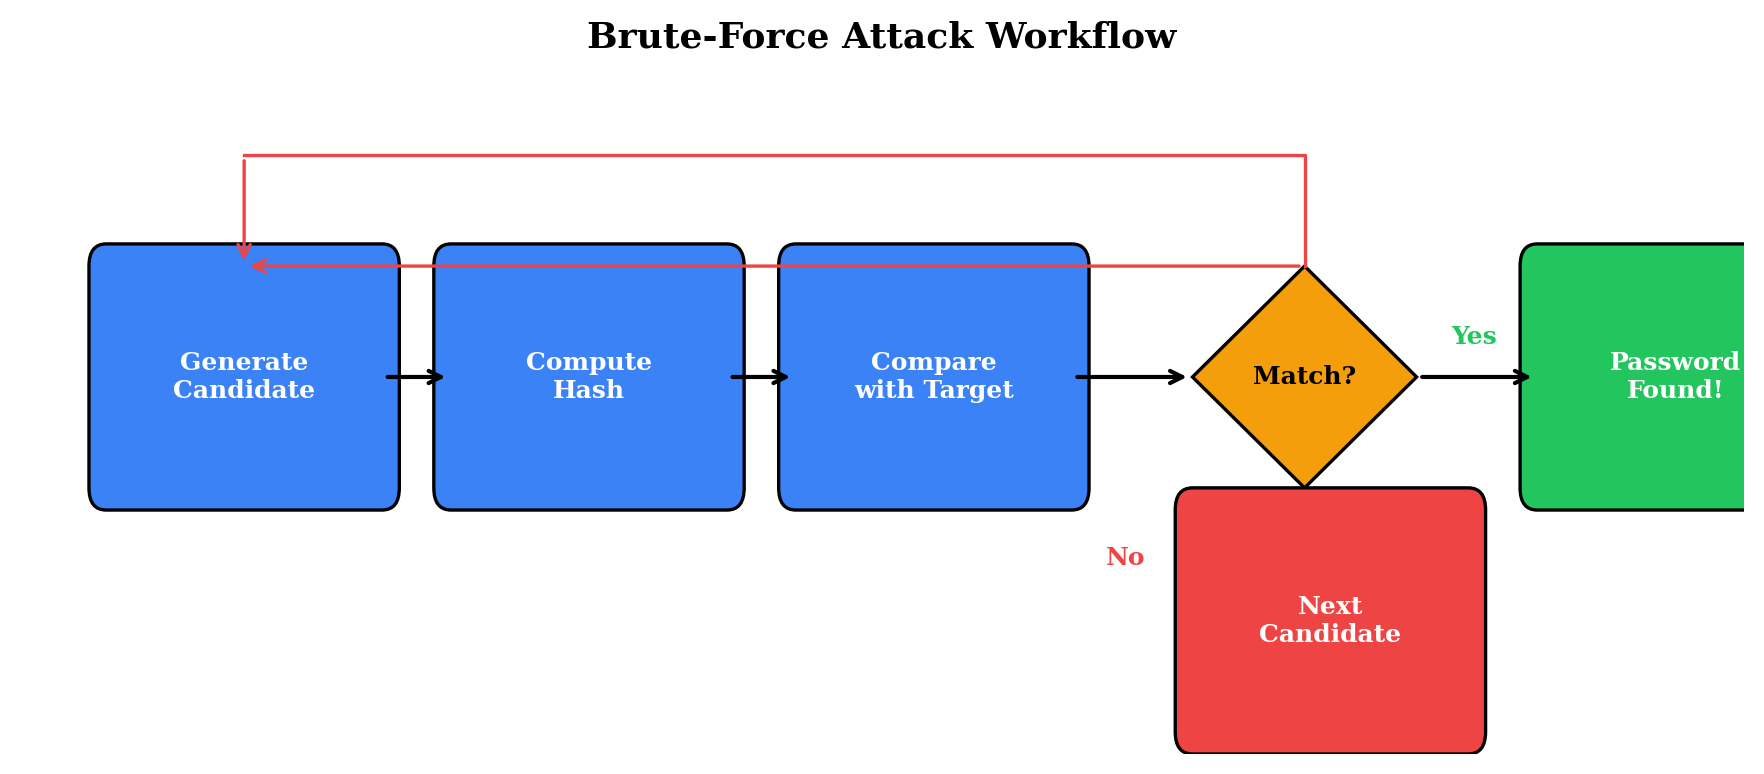
\includegraphics[width=0.85\textwidth]{figures/brute_force_workflow.png}
    \caption{Workflow of a brute-force attack.}
    \label{fig:brute_force}
\end{figure}

The time required for a brute-force attack grows exponentially with password length. This exponential relationship is the primary motivation for the length scoring dimension in the evaluation algorithm: longer passwords receive higher scores because they are exponentially harder to crack by exhaustive search.

\subsection{Dictionary Attacks}

A dictionary attack improves upon brute-force by using a pre-compiled list of likely passwords (a ``dictionary'') rather than trying every possible combination. The dictionary typically contains common passwords, words from natural language, and known leaked credentials. More sophisticated dictionary attacks apply mutation rules to each dictionary entry---capitalising the first letter, appending digits, replacing letters with similar-looking symbols (leetspeak), and combining multiple words.

\begin{figure}[H]
    \centering
    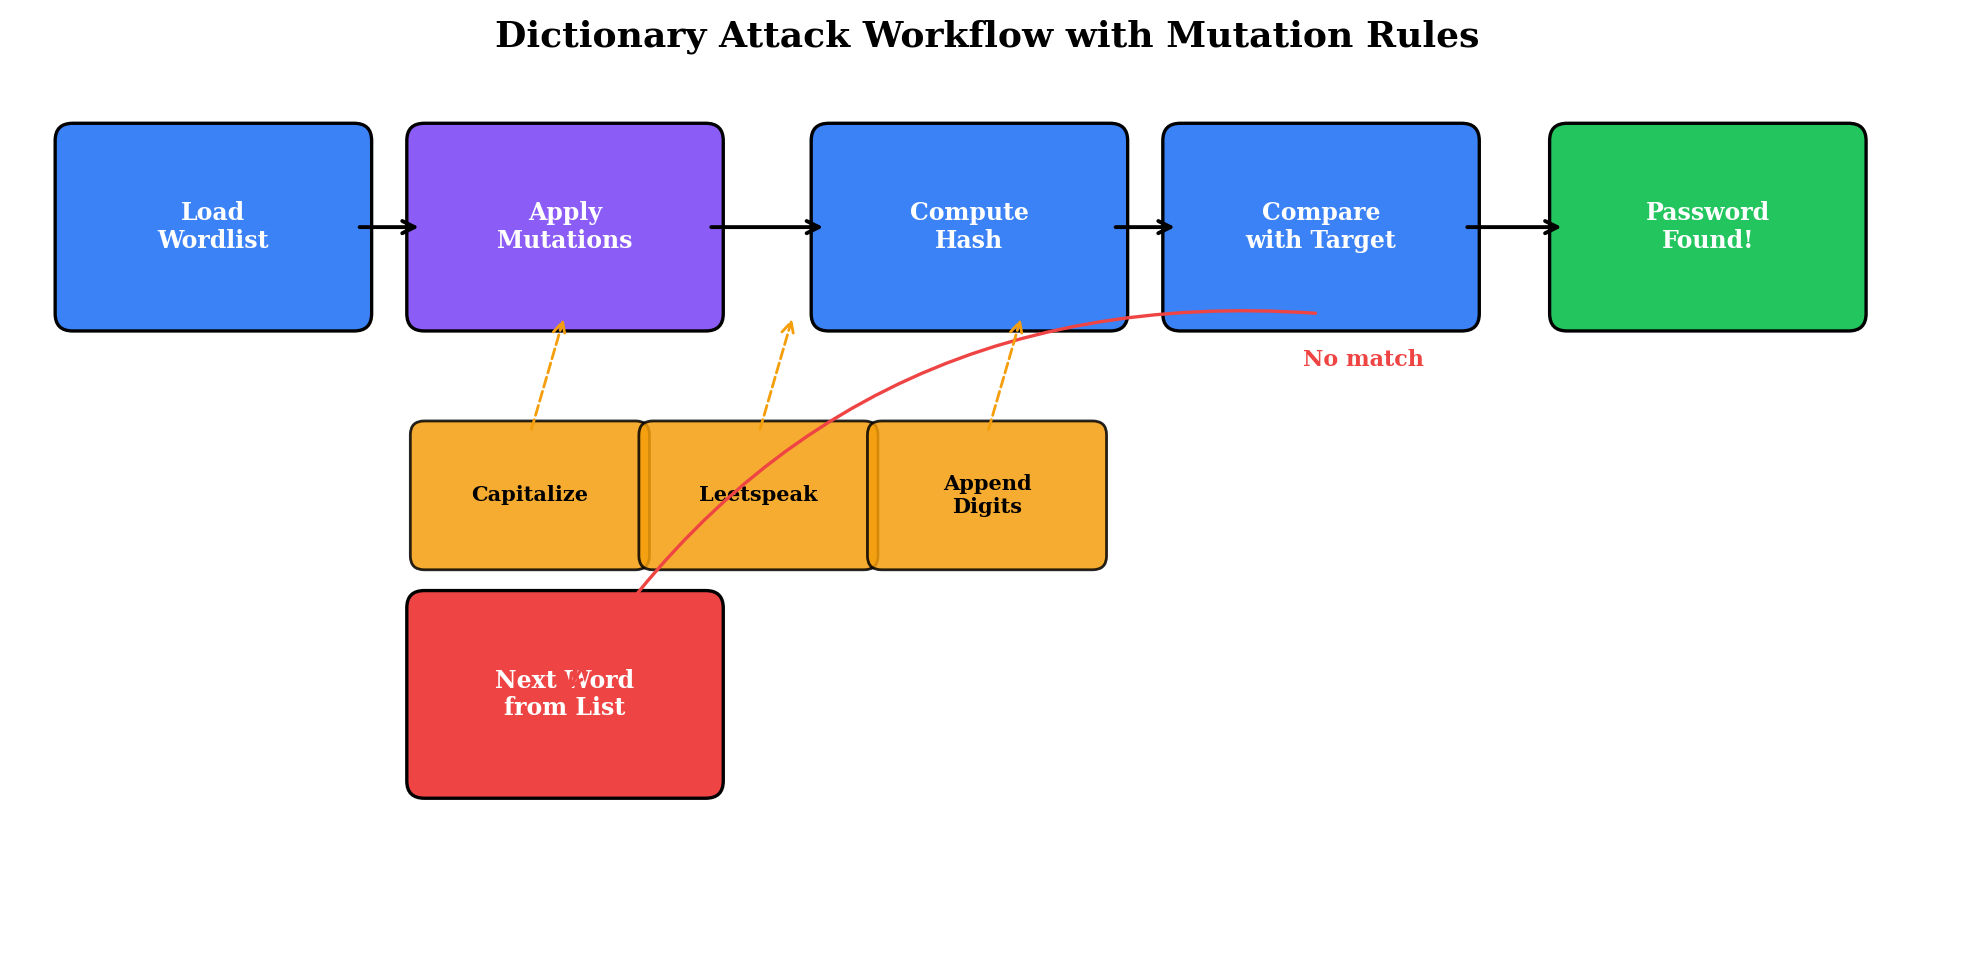
\includegraphics[width=0.85\textwidth]{figures/dictionary_attack_workflow.png}
    \caption{Workflow of a dictionary attack with common mutation rules.}
    \label{fig:dictionary_attack}
\end{figure}

Dictionary attacks are highly effective because most users choose passwords that follow predictable patterns. Wheeler demonstrated that the zxcvbn strength estimator, which models common password patterns, can crack many supposedly ``strong'' passwords far more efficiently than brute-force alone \cite{wheeler2016}. This motivates the dictionary comparison and Levenshtein similarity dimensions in the evaluation algorithm.

\subsection{Credential Stuffing}

Credential stuffing is an attack in which usernames and password pairs leaked from one breach are systematically tested against other online services. The attack exploits the widespread practice of password reuse: if a user employs the same password on multiple sites, a single breach compromises all of their accounts.

\begin{figure}[H]
    \centering
    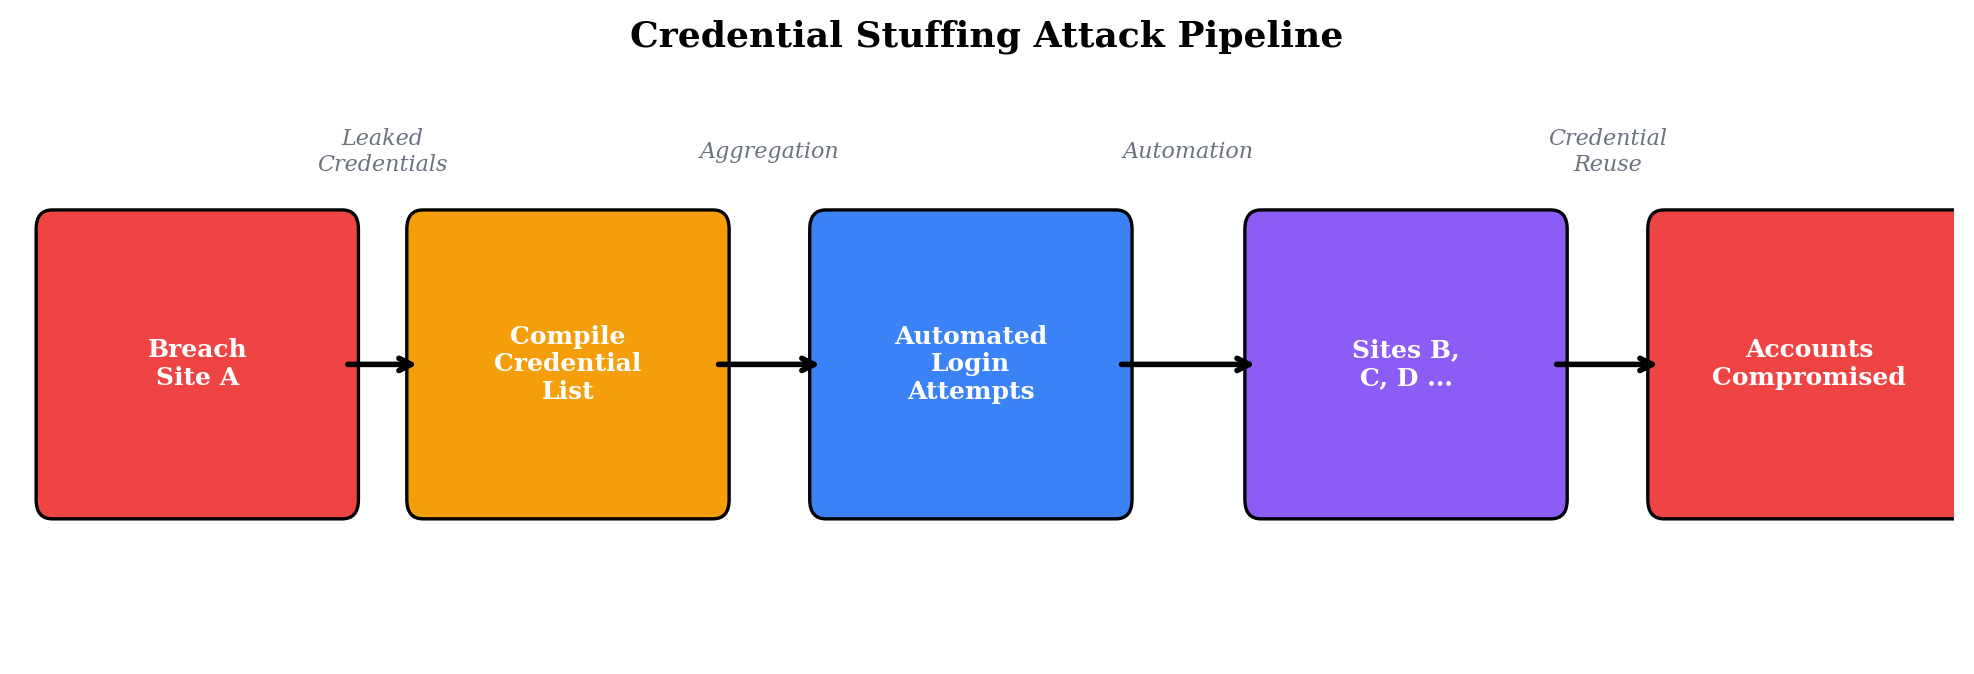
\includegraphics[width=0.85\textwidth]{figures/credential_stuffing_pipeline.png}
    \caption{Pipeline of a credential stuffing attack.}
    \label{fig:credential_stuffing}
\end{figure}

Credential stuffing attacks have been implicated in numerous high-profile incidents, including the Zoom breach of 2020, where attackers used credentials leaked from earlier breaches to access Zoom accounts \cite{verizon2024}. While the evaluation tool cannot directly prevent credential stuffing (which is a behavioural issue rather than a technical one), it can encourage users to create unique passwords by highlighting the risks of common and reused credentials.

\subsection{Rainbow Table Attacks}

Rainbow tables are pre-computed lookup tables that map cryptographic hash values to their corresponding plaintext passwords. Instead of computing the hash for each candidate password during an attack, the attacker simply looks up the stolen hash in the rainbow table. This approach trades storage space for computation time and is extremely efficient against unsalted password hashes.

Modern systems mitigate rainbow table attacks by using salted hashes (appending a random value to each password before hashing), which renders pre-computed tables useless. However, rainbow tables remain relevant for legacy systems that store unsalted hashes, and their existence underscores the importance of ensuring that even if a hash is stolen, the underlying password should be sufficiently complex to resist all attack methods.

\clearpage

\section{Real-World Examples of Password Breaches}

I also reviewed notable cybersecurity incidents that demonstrated the consequences of weak passwords and poor credential management:

\begin{itemize}
    \item \textbf{LinkedIn (2012):} Over 117 million passwords were leaked due to inadequate password hashing and users choosing simple combinations like ``123456.''\\
    The LinkedIn breach highlighted not only weak user passwords but also the risks of inadequate hashing mechanisms, allowing attackers to recover millions of credentials efficiently.

    \item \textbf{Facebook (2019):} Hundreds of millions of user passwords were stored in plaintext and accidentally logged in internal systems accessible to thousands of employees. While there was no confirmed large-scale external leak, it exposed how poor internal password handling can create serious insider and data exposure risks.\\
    This incident showed that strong user passwords are not sufficient on their own; organisations must also enforce secure storage practices (e.g., salted hashing) and strict access controls to prevent exposure from misconfigurations and internal tooling.

    \item \textbf{Zoom (2020):} During the early COVID-19 pandemic, attackers used ``credential stuffing'' with passwords leaked from older breaches to break into Zoom accounts and meetings, taking advantage of users who reused passwords across services.\\
    The Zoom incidents demonstrated how password reuse turns one breach into many, emphasising the need for unique passwords per site and support for multi-factor authentication to limit the impact of credential stuffing.

    \item \textbf{Colonial Pipeline (2021):} Ransomware operators accessed a VPN account using a compromised password that was found in a previous data breach and reportedly not protected by multi-factor authentication. The attack disrupted fuel supply across the U.S.\ East Coast.\\
    This case illustrated how a single exposed and reused password, combined with a lack of MFA on remote access, can have real-world physical and economic consequences far beyond the IT environment.

    \item \textbf{NVIDIA (2022):} An attacker group claimed to have accessed internal systems and leaked employee credentials and certificates. Password reuse and weak internal credential practices were reported as contributing factors, enabling deeper access once an initial foothold was gained.\\
    The NVIDIA incident underscored how weak or reused internal passwords can allow lateral movement inside corporate networks, turning one compromised account into widespread access to sensitive intellectual property.

    \item \textbf{LastPass (2022--2023):} An engineer's home machine was compromised, and an account protected by a master password was targeted. While the immediate cause was not a simple weak password list, the incident reignited concerns about master passwords, password vault security, and user password hygiene for the vault itself.\\
    The LastPass breach highlighted that even when password managers are used, the strength of the master password (and additional factors like MFA and device security) is critical, since compromising a single high-value credential can expose many others.

    \item \textbf{MOVEit-related credential attacks (2023):} In parallel with exploiting MOVEit vulnerabilities, threat actors also attempted to use previously leaked or weak credentials to access related infrastructure and accounts, combining software flaws with poor password practices.\\
    These campaigns showed how attackers increasingly blend vulnerability exploitation with credential-based attacks, meaning weak or reused passwords make organisations far more vulnerable even when patching cycles improve.
\end{itemize}

These examples reinforce the need for stronger user education, unique and complex passwords, multi-factor authentication, and secure organisational handling of credentials---which is precisely what I aimed to address through my project.


\section{Password Strength Evaluation Methods}

While studying password security, I came across several common methods used to measure password strength:

\begin{itemize}
    \item \textbf{Rule-based analysis:} Evaluates whether a password meets specific conditions (e.g., minimum length, inclusion of uppercase letters, numbers, and symbols). This approach is simple and transparent but often fails to capture deeper weaknesses such as dictionary words or predictable patterns.
    \item \textbf{Entropy-based analysis:} Estimates password unpredictability using information theory \cite{shannon1948}. Higher entropy values usually mean stronger passwords, but entropy alone does not account for patterns or dictionary words that may be tried first by attackers.
    \item \textbf{Dictionary comparison:} Checks if a password appears in known leaked datasets or common password lists. This method directly addresses the most likely attack strategy but does not evaluate structural properties like length or diversity.
    \item \textbf{Machine learning approaches:} More advanced models attempt to predict password strength using neural networks trained on large datasets \cite{melcher2016, castelluccia2012}. While effective, they are more complex to implement and operate as ``black boxes,'' making it difficult to explain the reasoning behind a particular strength rating.
\end{itemize}

For my project, I decided to combine the first three methods---rule-based checks, entropy calculation, and dictionary comparison---into a hybrid evaluation algorithm that balances simplicity, accuracy, and transparency. The hybrid approach addresses a key limitation of each individual method: rule-based checks miss patterns, entropy misses dictionary words, and dictionary checks miss structural weaknesses. By combining all three, the tool provides a more comprehensive assessment.


\section{Entropy and Password Strength}

Entropy represents the amount of unpredictability or randomness in a password. In information theory, it is measured in bits using the following formula, as introduced by Shannon \cite{shannon1948}:

\begin{equation}
H = L \times \log_2 N
\end{equation}

where $L$ is the password length and $N$ is the number of possible characters per position (for example, 26 for lowercase letters, 10 for digits, etc.). Higher entropy values correspond to more secure passwords.

\textbf{Intuitive explanation of log₂ and bits:}
The logarithm base 2 (log₂) measures how many times you need to double 1 to reach a value, or equivalently, how many binary decisions (bits) are needed to represent a number. Each bit of entropy represents a doubling of the guess space required to crack the password via brute-force.
\begin{itemize}
    \item 1 bit = 2 possibilities (0 or 1) -- requires 1 guess on average to crack
    \item 2 bits = 4 possibilities (00, 01, 10, 11) -- requires 2 guesses on average
    \item 10 bits = 1,024 possibilities -- requires 512 guesses on average
    \item 20 bits = 1,048,576 possibilities -- requires 524,288 guesses on average
    \item 30 bits = 1,073,741,824 possibilities -- requires 536,870,912 guesses on average
    \item 40 bits = 1 trillion possibilities -- requires 500 billion guesses on average
\end{itemize}
For example, an 8-character password using only lowercase letters has approximately:

\begin{equation}
H = 8 \times \log_2 26 \approx 37.6 \text{ bits}
\end{equation}

This means an attacker would need to try, on average, 2³⁷·⁶/2 ≈ 2³⁶·⁶ ≈ 100 billion guesses to crack it via brute-force.

While one including uppercase letters, digits, and symbols could exceed 60 bits---offering much stronger protection against brute-force attacks.

Table~\ref{tab:entropy_charset} provides a comprehensive comparison of entropy values across different password lengths and character set compositions, illustrating how both length and character diversity contribute to password strength.

\begin{table}[H]
\centering
\caption{Password entropy (bits) by length and character set composition.}
\label{tab:entropy_charset}
\begin{tabularx}{\textwidth}{ccccc}
\toprule
\textbf{Length} & \textbf{Lowercase only} & \textbf{+ Uppercase} & \textbf{+ Digits} & \textbf{+ Symbols} \\
 & ($N = 26$) & ($N = 52$) & ($N = 62$) & ($N = 94$) \\
\midrule
6  & 28.2  & 34.3  & 35.6  & 39.3  \\
8  & 37.6  & 45.7  & 47.5  & 52.4  \\
10 & 47.0  & 57.2  & 59.4  & 65.5  \\
12 & 56.4  & 68.6  & 71.3  & 78.6  \\
16 & 75.2  & 91.5  & 95.1  & 104.8 \\
\bottomrule
\end{tabularx}
\end{table}

The table clearly demonstrates that both length and character set diversity independently contribute to entropy, and that their combined effect is multiplicative. A 12-character password using all four character categories (78.6 bits) is roughly $2^{26}$ (approximately 67 million) times harder to crack by brute-force than a 12-character lowercase-only password (56.4 bits).

\begin{figure}[H]
    \centering
    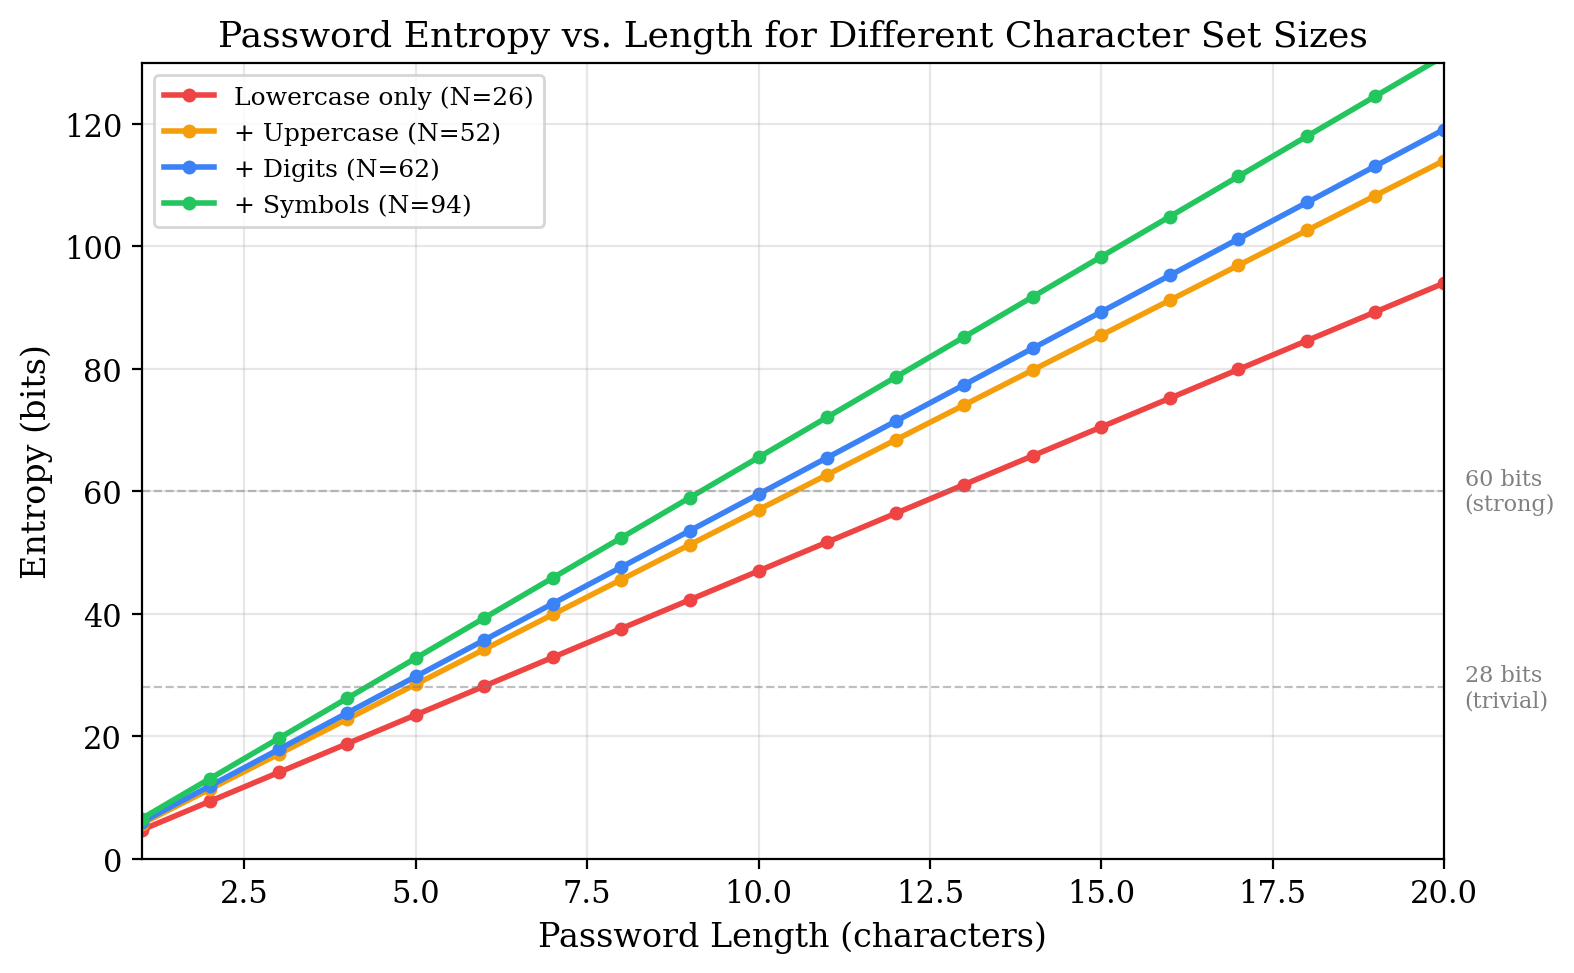
\includegraphics[width=0.85\textwidth]{figures/entropy_vs_length_graph.png}
    \caption{Entropy as a function of password length for four character set compositions.}
    \label{fig:entropy_graph}
\end{figure}

Consider a concrete comparison: the password \texttt{abcdefgh} (8 lowercase characters) has an entropy of approximately 37.6 bits, while the password \texttt{aB1!xY9\#} (8 characters mixing all categories) has an entropy of approximately 52.4 bits. Despite having the same length, the mixed-charset password is roughly $2^{14.8} \approx 28{,}000$ times harder to crack by brute-force. This example illustrates why both length and diversity are essential dimensions in a password strength evaluation model.

\textbf{Worked crack time examples:}
Assuming an attacker capable of 10¹⁰ guesses per second (10 billion/second, realistic for modern GPU cracking):
\begin{itemize}
    \item \texttt{abcdefgh} (37.6 bits): Average crack time = 2³⁷·⁶ / 2×10¹⁰ ≈ 100 billion ÷ 20 billion = 5 seconds
    \item \texttt{aB1!xY9\#} (52.4 bits): Average crack time = 2⁵²·⁴ / 2×10¹⁰ ≈ 4.5 million billion ÷ 20 billion ≈ 225,000 seconds ≈ 2.6 days
    \item \texttt{TestPass123!} (72.1 bits): Average crack time = 2⁷²·¹ / 2×10¹⁰ ≈ 50 billion billion ÷ 20 billion ≈ 2.5 billion seconds ≈ 79 years
    \item Generated 16-char password (104.8 bits): Average crack time = 2¹⁰⁴·⁸ / 2×10¹⁰ ≈ 20,000 billion billion billion ÷ 20 billion ≈ 18,000 centuries
\end{itemize}
This shows why entropy alone doesn't determine practical security---a password like \texttt{password} (which would have 37.6 bits if truly random) falls instantly to dictionary attacks despite the brute-force estimate of 5 seconds.


\section{Existing Tools and Standards}

Several password checkers and guidelines influenced my approach. Table~\ref{tab:tools_comparison} presents a formal comparison of the most relevant tools and standards.

\begin{table}[H]
\centering
\caption{Comparison of password strength evaluation tools and standards.}
\label{tab:tools_comparison}
\begin{tabularx}{\textwidth}{lcccc}
\toprule
\textbf{Tool / Standard} & \textbf{Method} & \textbf{Online / Offline} & \textbf{Breach Database} & \textbf{Open Source} \\
\midrule
Our tool & Hybrid (rules + entropy + patterns + dictionary) & Offline & Local list (181 entries) & Yes \\
zxcvbn \cite{wheeler2016} & Pattern matching + entropy & Offline & Built-in frequency list & Yes \\
Have I Been Pwned \cite{hibp2021} & Breach database lookup & Online & 600M+ entries & Partially \\
NordPass Checker \cite{nordpass2024} & Rule-based + breach data & Online & Proprietary & No \\
NIST SP 800-63B \cite{nist2017} & Guidelines (blacklist-based) & N/A & Recommends breach check & N/A \\
\bottomrule
\end{tabularx}
\end{table}

The \textbf{NIST Digital Identity Guidelines (SP 800-63B)}, published in 2017 and updated in 2020, represent a significant shift in password policy philosophy \cite{nist2017}. The guidelines recommend:

\begin{itemize}
    \item Avoiding arbitrary composition rules (e.g., ``must contain at least one uppercase letter and one digit'') that lead to predictable patterns,
    \item Using blacklist-based validation, checking passwords against known compromised password lists,
    \item Allowing all printable ASCII characters and Unicode characters,
    \item Permitting paste functionality to support password managers,
    \item Not requiring periodic password changes unless there is evidence of compromise.
\end{itemize}

\begin{figure}[H]
    \centering
    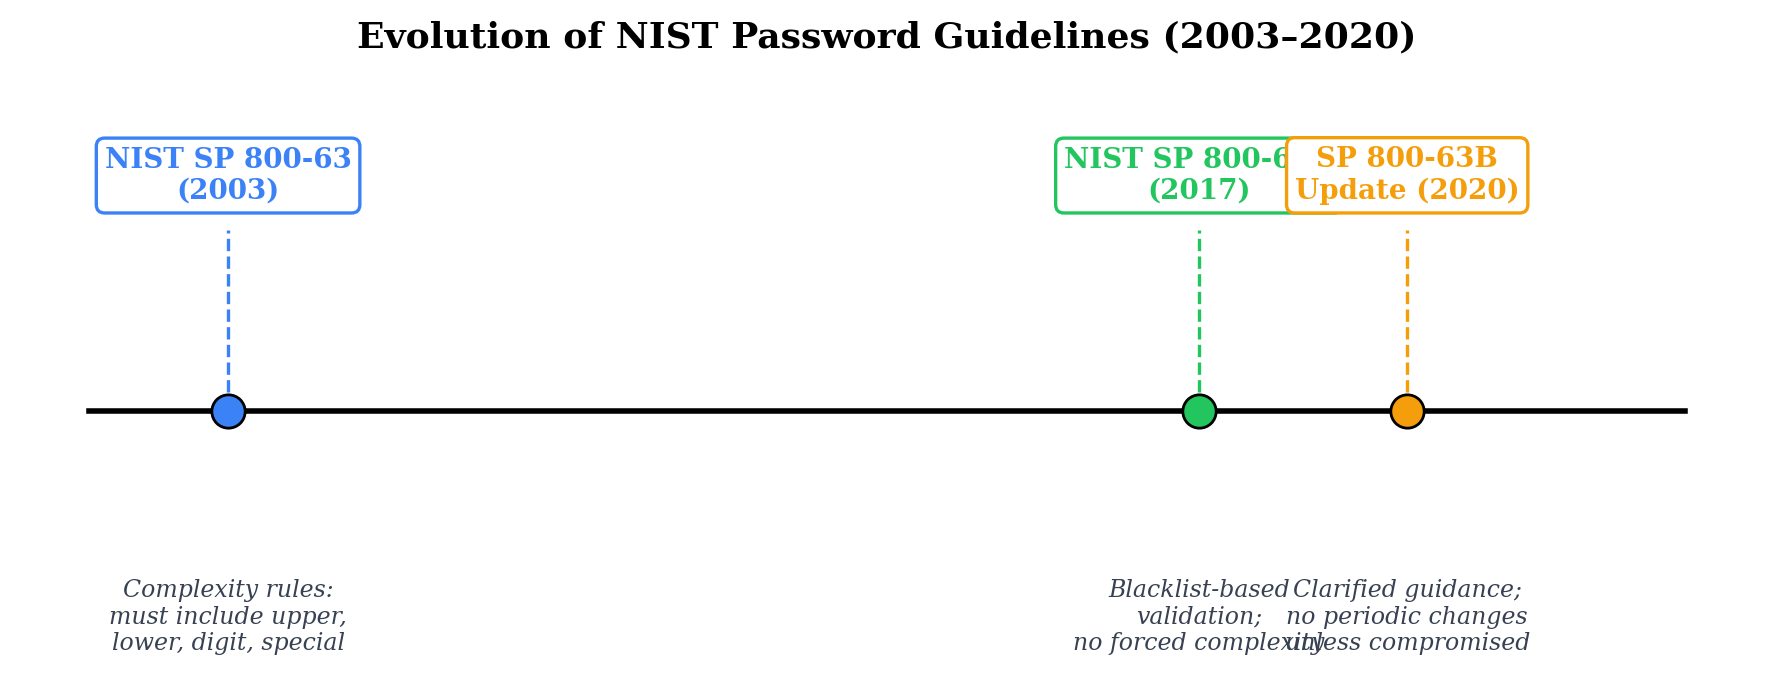
\includegraphics[width=0.85\textwidth]{figures/nist_guidelines_timeline.png}
    \caption{Evolution of NIST password guidelines from complexity rules to blacklist-based validation.}
    \label{fig:nist_timeline}
\end{figure}

By analyzing these existing tools and standards, I learned that effective password evaluation should combine mathematical rigor with user-friendly feedback — a balance I aimed to achieve in my own implementation. The NIST guidelines, in particular, motivated my decision to include dictionary comparison and to keep the scoring model transparent through named constants, so that users can understand why a particular score was assigned rather than relying on a ``black box'' assessment.


\section{Summary}

In this chapter, I reviewed the theoretical foundations of password security and evaluation. I discussed the role of passwords in modern authentication, identified common vulnerability types and their security impact, described the mechanisms of the four principal categories of password attacks, examined real-world breach examples, reviewed the four main approaches to password strength evaluation, provided a detailed analysis of entropy and its relationship to password strength, and compared existing tools and standards.

The key insight from this review is that no single evaluation method is sufficient on its own: rule-based checks miss patterns, entropy misses dictionary words, and dictionary checks miss structural weaknesses. This motivates the hybrid approach adopted in this thesis, which combines all three methods into a single, transparent scoring model. The next chapter describes the methodology used to implement this hybrid approach.